\section{Discussion: Implications for Interaction Design in Built Environments}
\label{sec:ch5-discussion}

This study investigated how biophilic experiences can inform the design of interactive indoor environments through three expert speculative design sessions and a multi-layered analysis (\autoref{fig:study-overview}). Collectively, the contributions form the first biophilic interaction design framework for HCI and HBI, comprising three layers: (1) seven \emph{biophilic design dimensions} that map the experiential design space (Layer~1; RQ1); (2) seven \emph{biophilic interaction design values} that capture the normative orientations guiding design reasoning (Layer~2; RQ2); and (3) six \emph{biophilic interaction forms} that abstract recurring logics of bodily interaction with technologically mediated environments (Layer~3; RQ3). Together, these layers provide a unified resource for comparative analysis, generative design exploration, and translation into interaction design practice.

Below, we discuss what the layers and the framework as a whole contribute to interaction design (IxD) and Human--Building Interaction (HBI), outline implications for prototyping and evaluation, and reflect on limitations and future work.



\subsection{Design Contributions: Formalising the Biophilic Interaction Design Space Dimensions}
\label{subsec:ch5-layer1-discussion}
We contribute a design-space map for biophilic interaction in indoor environments for HBI and IxD researchers, comprising seven analytic dimensions and associated codes (\autoref{fig:biophilic-map}). The dimensions specify \emph{which experiential qualities} were foregrounded in experts’ reasoning, while the codes specify \emph{how those qualities were articulated} in practice. 

The dimensions surface design concerns that remain under-specified in HBI discourse. Notably, \emph{Interaction Type} and \emph{Spatial Context} frame biophilic interaction as embodied engagement arising from routine movement and dwelling in specific architectural settings (e.g. pausing in thresholds, lingering in alcoves), rather than through explicit user inputs such as submitting thermal preferences via an app~\cite{kudryashova2020interactive, clear2013understanding} or touching responsive furniture (e.g. occupancy-conveying doors ~\cite{economidou2021no}). In addition, \emph{Natural Reference} makes ecological inspiration an explicit design choice: while biophilic work in buildings is often operationalised through plant installations or visual ``green'' cues~\cite{buechley2010living, feng2019livenature}, our map surfaces a broader set of ecological sources (e.g. terrain, water, and atmospheric variation), enabling future work to deliberately expand what ``counts'' as biophilic inspiration beyond vegetation. Finally, prior wellbeing-oriented building research often centres on stress reduction~\cite{feng2019livenature, wang2014livenature}, restoration~\cite{angelini2015multisensory} and socialisation~\cite{nguyen2023engaging, nguyen2024adaptive}; in contrast, \emph{Affective Aim} captures a much wider set of emotions foregrounded in expert reasoning (e.g. curiosity, vitality, connection, and mental reset alongside calm).

Supported by \autoref{fig:biophilic-map}, the map makes these configurations visible at scale, showing where the corpus concentrates or disperses and how qualities co-occur across dimensions. It provides a shared reference point for future work: new concepts can be situated relative to prior configurations, under-explored regions can be identified, and the structure itself can be extended as the field evolves.

\subsection{Normative Contributions: Value Orientations for Biophilic Interaction}
\label{subsec:ch5-layer2-discussion}
The seven biophilic design values (\autoref{sec:ch5-layer2}) capture recurrent \emph{experiential orientations} through which experts exercised design judgement when reasoning about biophilic interaction in indoor environments. They help articulate what designers may intentionally choose to leave unresolved, unoptimised, or non-personalised when designing for experiential richness.

These values extend HBI---IxD research by consolidating under-articulated concerns and introducing value orientations largely absent from building-focused discourse. \emph{Sensory Ecology}, \emph{Attentional Ease}, and \emph{Proprioceptive Engagement} resonate with prior HCI work on multisensory interaction (e.g. exploring sound, smell, and cross-modal perception~\cite{andres2023human,becsevli2024smell}), embodied experience (e.g. treating the body as a site of interaction~\cite{van2018skin}), and soma-based design (e.g. designing for felt bodily states~\cite{damen2021office}). Here, however, these concerns are re-situated at architectural scale and within everyday indoor environments, rather than interfaces, artefacts, or personal devices.

In contrast, \emph{Irreversibility}, \emph{Unknowability}, \emph{Non-Reciprocity}, and \emph{Collective Liability} surface orientations rarely foregrounded in HBI. These values articulate persistence (e.g. experiences that accumulate and cannot be reset), ambiguity (similar to work exploring ``magical'' behaviour as experiential~\cite{economidou2021moving}), asymmetry (e.g. occupants maintain an indoor weather system that is responsive to environmental conditions, sustaining a non-reciprocal relation~\cite{gaver2013indoor}), and shared consequence (e.g. collective responsibility enacted through a shared artefact, such as a plant that must be jointly cared for by occupants~\cite{loh2010please}). Such qualities resist being framed as system goals, performance metrics, or user benefits, yet were central to how experts evaluated the authenticity, depth, and ecological credibility of biophilic interaction.

\subsection{Design Contributions: Biophilic Interaction Forms}
\begin{figure*}[!ht]
    \centering
    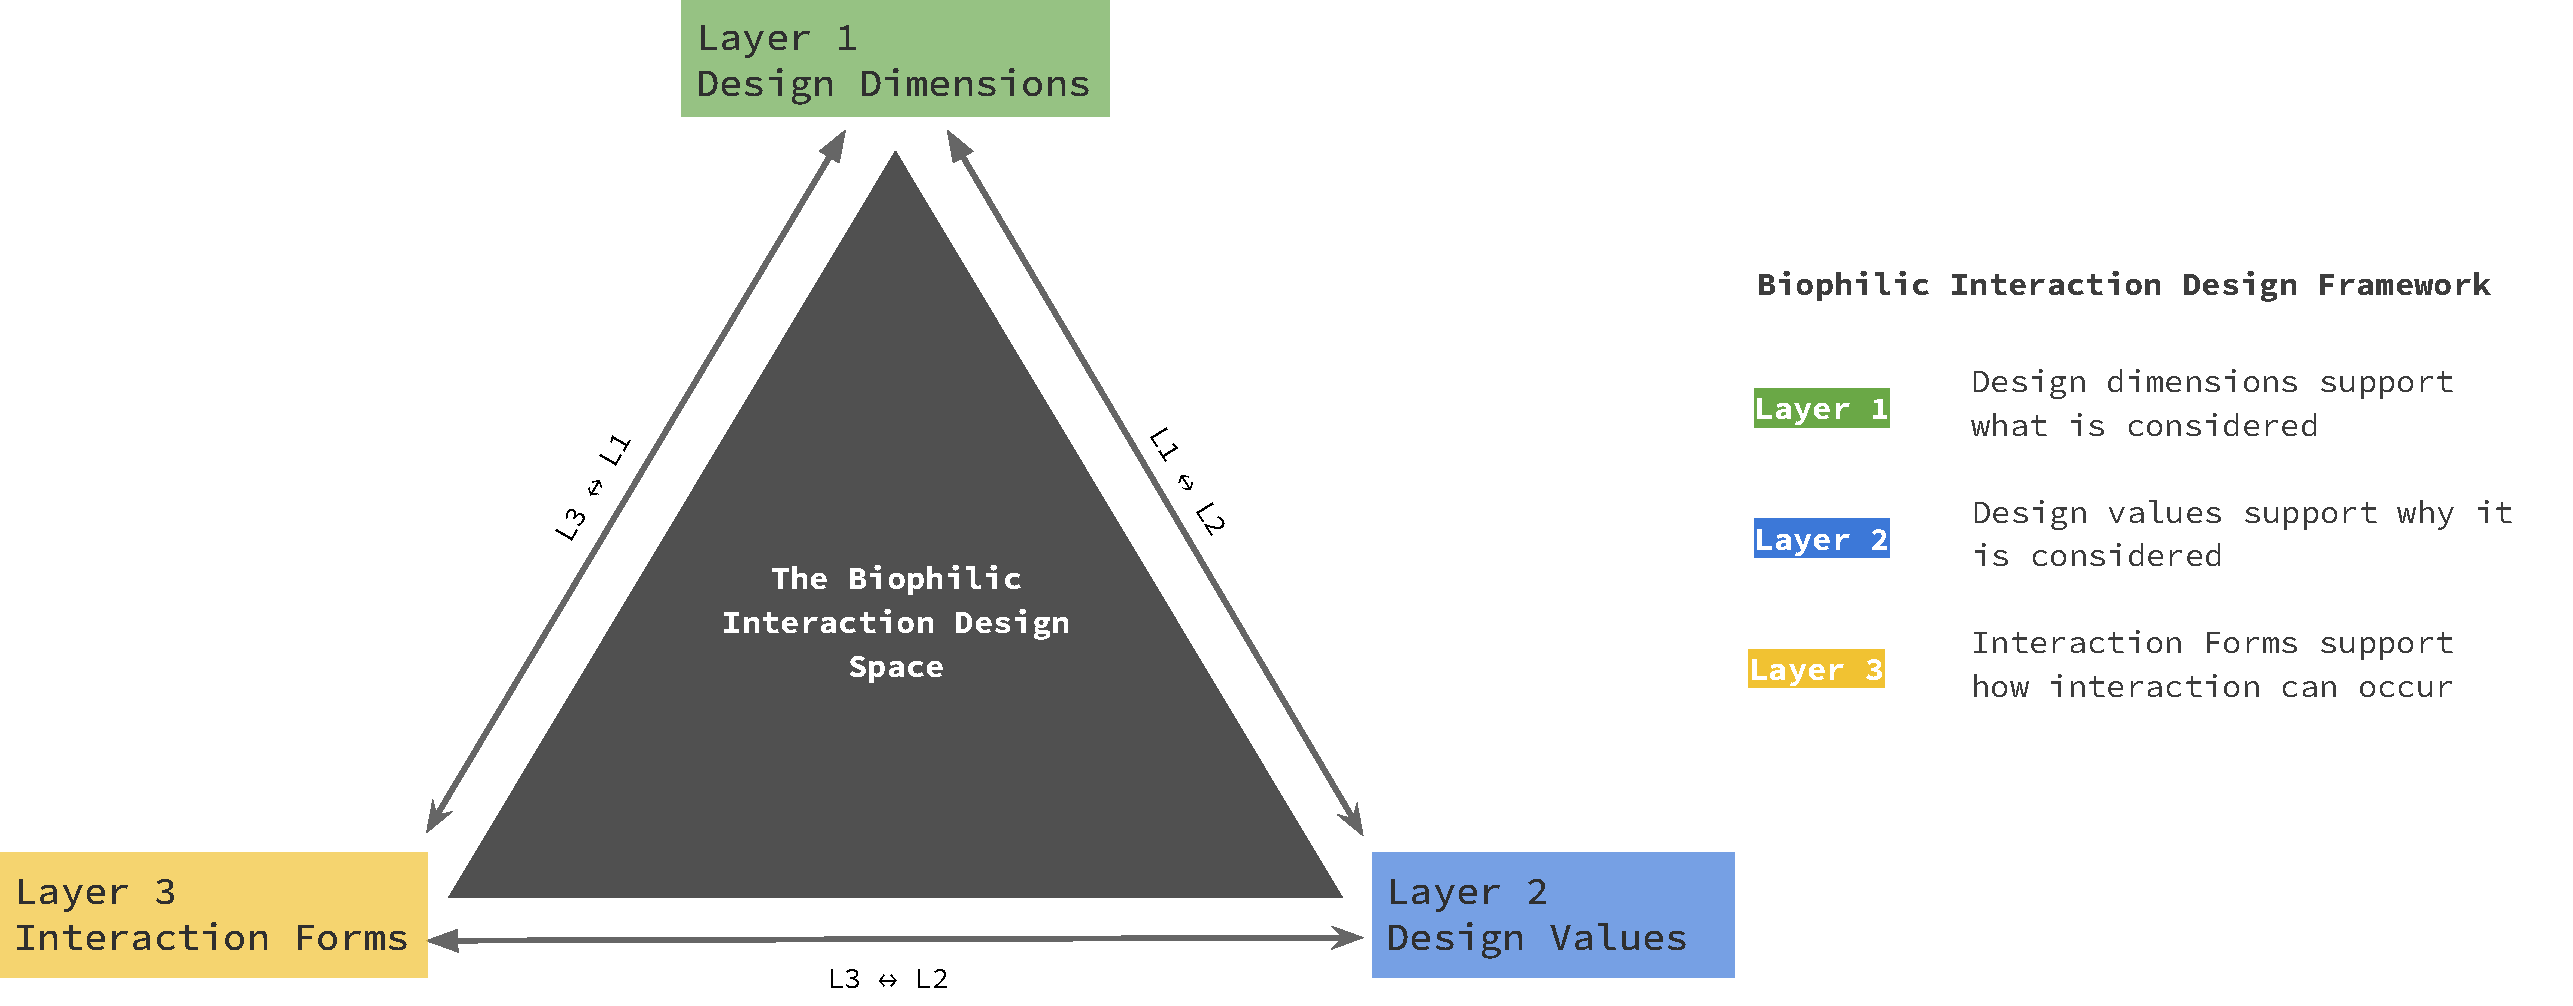
\includegraphics[width=\linewidth]{images/discussion/dis26-framework (1).pdf}
    \caption{Biophilic Interaction Design Framework comprises three analytically distinct but conceptually connected layers: design dimensions (Layer~1), design values (Layer~2), and interaction forms (Layer~3). Each layer captures a different aspect of biophilic interaction design: what is configured in the environment, why it is configured in particular ways, and how interaction unfolds through bodily and spatial engagement. The layers are not hierarchical and do not operate as a fixed sequence. Instead, they form a relational structure in which each layer can inform and constrain the others. Designers may enter the framework from any layer—starting, for example, from an intended interaction form, a set of values, or a spatial configuration—and iteratively move between layers to develop and refine design concepts. This relational organisation enables the framework to support both analysis and generative design.}
    \Description{A conceptual diagram of the Biophilic Interaction Design Framework consisting of three analytically distinct but interconnected layers: Design Dimensions (what is configured), Design Values (why it is configured), and Interaction Forms (how interaction unfolds). The layers are arranged in a non-hierarchical, relational structure with bidirectional connections, indicating that designers can enter from any layer and iteratively move between them to analyse or develop biophilic interaction concepts.}
    \label{fig:framework}
\end{figure*}

\label{subsec:ch5-layer3-discussion}
The six biophilic interaction forms, \emph{Anchoring}, \emph{Synchronising}, \emph{Dwelling}, \emph{Inferring}, \emph{Withholding}, and \emph{Accepting} (cf. \autoref{sec:ch5-layer3}) articulate novel or alternate ways \emph{in which interaction occurs}. They function as interaction-level abstractions: open-ended enough to support multiple instantiations, yet specific enough to guide design logic and system behaviour at architectural scale. 

Across prior research on interactive experiences in indoor environments (most recently synthesised in a scoping review~\cite{rao2025smart}), interaction is predominantly organised around a narrow set of recurring logics. Occupants typically interact by \emph{configuring} environmental parameters such as light or temperature through interfaces~\cite{alavi2017comfort,kudryashova2020interactive,clear2013understanding}; by \emph{monitoring} system state or environmental conditions via dashboards and visualisations~\cite{margariti2024evaluating}; or by \emph{reacting} to immediate system responses triggered through presence or movement~\cite{vallgaarda2014dress}. Even when work targets affective~\cite{gaver2006history}, social~\cite{petersen2007squeeze}, or speculative aims~\cite{gough2021speculating}, interaction is typically structured around discrete events that render system behaviour perceivable or actionable (e.g. learning how building sensors use personal data~\cite{schnadelbach2019adaptive}).

In contrast, the biophilic interaction forms reframe interaction around how occupants remain with, move through, and attune to evolving environmental conditions over time. \emph{Anchoring} and \emph{Dwelling} foreground lingering, bodily contact, and accumulated presence, challenging event-based models of interaction~\cite{hansen2009pendaphonics}. \emph{Synchronising} shifts interaction from individual action to alignment with shared environmental rhythms rather than immediate or personalised response~\cite{yu2018delight}. \emph{Inferring} centres embodied sense-making through indirect multisensory cues rather than explicit displays or dashboards~\cite{marques2020real}. \emph{Withholding} and \emph{Accepting} depart most sharply from dominant paradigms by resisting invitation, control, or optimisation: interaction unfolds through distance, exposure, or the decision to remain with unbuffered conditions.

\emph{Withholding} in particular frames non-responsiveness as an intentional design quality. Occupants must adjust to or remain with environmental conditions without expecting control or reciprocity. This puts \emph{Withholding} in tension with dominant paradigms of responsiveness and personalisation where systems are expected to sense and adapt to user needs to minimise discomfort~\cite{alavi2017comfort}.  This aligns with values in Layer~2, particularly \emph{Non-Reciprocity}, \emph{Irreversibility}, and \emph{Unknowability}, where systems do not necessarily resolve or adapt to user input but instead sustain conditions that must be navigated or endured. In doing so, \emph{Withholding} expands the scope of interaction design by introducing the possibility of designing \emph{for non-action}, where meaning and experience emerge through what systems do not do. While Anchoring, Dwelling, and Synchronising resonate with prior work in embodied and soma-based interaction, our contribution lies in extending these concepts to architectural scale where interaction occurs through spatial conditions rather than discrete artefacts or interfaces.

Additionally, the illustrative system mechanisms associated with the interaction forms should not be interpreted as immediately deployable solutions. They function as speculations that make the interaction logic materially legible. Prior work on shape-changing interfaces, actuated environments, and ambient systems similarly highlights the difficulty of integrating fine-grained actuation, sensing, and material behaviour at scale~\cite{ishii2012radical, follmer2013inform, gaver2013indoor}. Several proposed mechanisms remain active areas of research and would require substantial advances in hardware integration, robustness, and coordination~\cite{lin2025wearable, chhaglani2023breatheasy, weyns2025architectural}. The contribution here is the articulation of interaction logics that can guide future technical exploration.

\paragraph{A Post-Personalised Model of Interactions in Indoor Environments.}
Across the interactions, sensing is presence-, movement-, duration-, and density-based. This is not a technical limitation. By avoiding reliance on biometric inference~\cite{gao2022understanding}, user profiles~\cite{bower2019impact}, or affect prediction~\cite{swaminathan2021tactile}, the forms remain legible at architectural scale and reduce the need for intimate data collection in everyday environments. Here, ``intelligence'' is the situational orchestration of shared conditions rather than personalised interpretation.



\subsection{Using the Biophilic Interaction Design Framework}
\label{subsec:ch5-integration}
The three layers form a relational framework rather than a fixed sequence. They capture complementary aspects of biophilic interaction design: \emph{what} is configured (dimensions), \emph{why} it is configured in particular ways (values), and \emph{how} interaction unfolds (forms). The layers are analytically distinct yet conceptually connected.

The framework supports multiple entry points. Designers may begin with an intended interaction form (e.g.~\emph{Dwelling}), then draw on relevant values and configure dimensions accordingly, or start from a spatial or sensory configuration and articulate the values and forms it enables. In this way, the framework connects experiential configuration, normative orientation, and interaction logic without prescribing a fixed order of use (\autoref{fig:framework}).

One way this can be operationalised is as follows: \textbf{(1) Select a biophilic interaction form} \emph{(Layer~3)} that reflects the intended mode of environmental interaction; \textbf{(2) identify relevant design values} \emph{(Layer~2)} to guide experiential decisions; and \textbf{(3) configure the experiential dimensions} \emph{(Layer~1)} that align with those interaction and value goals.



\paragraph{Worked Example.}
A research team plans to explore alternative non-visual wayfinding practices for indoor work environments. Focusing on how occupants orient themselves between quieter, social, and collaborative areas, they adopt the interaction form \emph{Inferring} (Layer~3), framing wayfinding as gradual sensory interpretation through movement and exposure. Guided by \emph{Sensory Ecology}, \emph{Attentional Ease}, and \emph{Unknowability} (Layer~2), the team identifies acoustics as the primary modality to explore (Layer~1). Rather than signalling destinations, they plan to investigate how acoustic character thickens, thins, or drifts without marking boundaries, forming continuous gradients that occupants learn to read over time by listening, slowing, or lingering. The aim is to probe how such acoustic variation can support orientation without instruction and how much ambiguity remains workable.


\subsection{Implications for Metrics and Evaluation}
\label{subsec:ch5-evaluation}
The findings imply that evaluating biophilic interaction cannot rely on traditional metrics such as usability, comfort ratings~\cite{alavi2019introduction, alavi2017comfort}, or individual preference satisfaction~\cite{abdalla2016decision}, valence and arousal scales~\cite{lottridge2011affective} alone. Because many forms operate through temporality, shared environmental conditions, and sensory coupling, evaluation must be reframed around new experiential criteria.

\paragraph{Evaluate temporal fit.}
Interaction forms such as \emph{Dwelling}, \emph{Synchronising}, and \emph{Accepting} centre on rhythm, delay, and sustained presence. The question is not whether systems respond quickly, but whether changes unfold at tempos that align with bodily attunement and everyday movement. Evaluation methods must capture trajectories over time, such as repeated walk protocols or trace-based interviews that surface noticing, habituation, or drift. This can be operationalised by measuring dwell time, movement tempo, and alignment between environmental change and activity transitions, rather than response speed or efficiency.

\paragraph{Evaluate legibility without instruction.}
Values like \emph{Attentional Ease}, \emph{Unknowability}, and \emph{Non-Reciprocity} call for interaction that is perceptible without demanding active attention. This implies that systems should support orientation or action without signage, alerts, or detailed instructions (e.g. ~\cite{swaminathan2021tactile}). Evaluation can assess whether occupants make ``good enough'' sense of a space through bodily inference and ambient exposure, e.g. confidence in wayfinding under reduced visual cues, comfort-with-uncertainty scales, and behavioural indicators such as pausing, rerouting, or hesitation. This can be assessed through users’ ability to orient and act without guidance, measured via wayfinding success, reliance on cues, and verbalised understanding of environmental conditions.

\paragraph{Evaluate collective interaction and negotiation.}
Forms like \emph{Withholding} and values such as \emph{Collective Liability} require attention to shared rather than personalised experience. The focus is on patterns of distribution, social comfort, and fairness of access. Evaluation approaches might include co-presence mapping and post-encounter group reflections that foreground negotiation, tolerance, and shared inhabitation (e.g. building walks~\cite{mitchell2020no, mitchell2020human}). This can be evaluated by observing patterns of shared use and reported experiences of fairness, coordination, and mutual adjustment.

\paragraph{Evaluate constrained sensing as an experiential affordance.}
Biophilic interaction forms intentionally rely on limited, observable signals—such as presence, movement, duration, and density—eschewing data-rich user models or affective inference. This repositions sensing constraints as design features that enable legibility and privacy in shared environments. Evaluation can explicitly compare systems with narrow versus expansive interpretive reach, attending to differences in perceived trust, environmental alignment, and cognitive or emotional load over time~\cite{dalton2020habitech, moran2013using, paraschivoiu2023postcards}. 

\subsection{Why Sound Was Not a Distinct Interaction Form: Lessons Learnt}
Session~3 was designed to foreground sound as a biophilic modality. Prompts and activities focused explicitly on outdoor sound experiences and how these change indoors. However, we did not enforce it as an exclusive design constraint and experts were free to interpret and develop their ideas according to their own disciplinary practices. This decision was intentional, allowing us to observe how sound would be taken up within architectural imagining.

\paragraph{What Occurred in the Session.}
Revisiting the transcripts, we found that sound was explicitly discussed for its layered, temporal, and affective qualities (cf.~\autoref{subsec:ch5-session3}). However, when experts moved into design, it got absorbed into spatial and material reasoning, becoming an acoustic property (e.g. absorption, diffusion, dampening) or an atmospheric enhancer (e.g. background water, ambient sound). As a result, sound occurred indirectly through form, material, and movement rather than a stand-alone interaction.

This observation aligns with how sound has historically been treated within architectural practice, where it is rarely designed as a discrete interaction but instead as a spatial condition. Architectural precedents ranging from reverberant worship spaces~\cite{mcmahon2013space} to concert halls engineered for acoustic diffusion~\cite{wheatley2007sound}, sound-masked offices~\cite{bruyninckx2023tuning, jacobsen2023living}, and recent work on sonic indoor environments~\cite{petersen2025sound, nabil2017interioractive} similarly treat sound as ambient and environmental. In this sense, the experts’ responses do not necessarily indicate a failure to engage with sound, but rather a faithful enactment of their disciplinary thinking: sound emerges from space, rather than being directly interacted with (also reflected upon by~\citet{fowler2015sounds}, despite calls for more multisensory approaches by Pallasmaa and Sheridan~\cite{pallasmaa2024eyes}). This has important implications for researchers in HBI and IxD working with experts in exploratory design settings. First, it highlights that expert participants will often reinterpret prompts through the epistemologies and practices of their field, even when alternative framings (e.g. interaction-centred perspectives from HCI) are introduced. Second, it suggests that resistance or deviation from the intended focus can itself be analytically productive, revealing underlying assumptions about what constitutes a ``designable'' element.\sidenote{We recognise that a more directive facilitation, such as enforcing sound as the primary interaction medium, may have led to more explicit sound-based interactions. However, it remains unclear whether such outcomes would reflect genuine architectural reasoning or artefacts of the imposed constraint.}



\subsection{Limitations and Future Work}
\label{subsec:ch5-limitations}
This work reflects our positional lens at the intersection of interaction design, HCI, and architectural practice, and has several limitations. First, the empirical material is grounded in speculative design sessions with a small number of architecture and design practices, primarily situated in European professional contexts. The paper therefore captures expert imaginaries and design reasoning about biophilic interaction, rather than how such concepts are perceived, negotiated, or sustained in everyday use. It also reflects only part of building practice, where interaction is shaped not only by architects and occupants but also by building managers and facility operators~\cite{mitchell2020no}. Architects and designers are well positioned to articulate atmospheric, spatial, and material possibilities, but may privilege conceptual coherence, subtlety, or ecological depth over practical legibility, accessibility, or ease of use. Some values and interaction forms surfaced here may therefore prove effortful, undesirable, or difficult to sustain in lived settings. The contribution should be understood as a design-facing articulation of biophilic interaction possibilities, not a validated account of occupant experience.

Second, the participant sample reflects a relatively homogeneous cultural and professional context, with all sessions conducted with European architecture practices. Although the paper opens with Haveli architecture to illustrate the broader diversity of biophilic design, the empirical basis of the framework is shaped by largely European expert imaginaries. The design dimensions, values, and interaction forms presented here are therefore not culturally neutral, but shaped by specific architectural traditions, climatic assumptions, and professional sensibilities. In other contexts, biophilic interaction may draw on different indoor–outdoor relations, material practices, or ecological and collective worldviews~\cite{rao2025designing}. The framework should thus be understood as one situated articulation rather than a universal account. Future work should examine how these layers evolve across diverse cultural and geographic contexts.

Next, the findings emerge from speculative, design-led inquiry rather than in-the-wild deployment. While this surfaced tacit, under-represented reasoning in smart building research, it limits insight into long-term use, habituation, breakdown, and organisational constraints such as accessibility, maintenance, and sustainability. A further limitation is that the framework has so far only been developed and applied within the expert workshops reported here. Its usability and generative capacity have not yet been evaluated with designers. Our future work is therefore applying the framework in independent design exercises to assess how it supports design exploration, what it foregrounds, and where it requires refinement.

Finally, the system mechanisms associated with the interaction forms were interpretively developed by the authors as illustrative examples. Future work will address these limitations through iterative prototyping and deployment. In particular, we are developing a sound-based biophilic system for office environments to evaluate \emph{Synchronising}, \emph{Dwelling}, and \emph{Accepting} under real-world conditions.


